\documentclass[fyp]{socreport}
\usepackage{bm}
\usepackage{fullpage}
\usepackage{url}
\usepackage{multirow}
\usepackage{graphicx}
\usepackage{amsthm}
\usepackage{amssymb}

\theoremstyle{definition}
\newtheorem{definition}{Definition}[section]
\theoremstyle{hypothesis}
\newtheorem{hypothesis}{Hypothesis}[section]

\begin{document}
\pagenumbering{roman}
\title{Leveraging Social Context in Fake News Detection with Graph Representation}
\author{Nguyen Van Hoang}
\projyear{2019/20}
\projnumber{H0791800}
\advisor{A/Prof. Min-Yen Kan, Dr. Kazunari Sugiyama}
\deliverables{
	\item Report: 1 Volume
	\item Source Code: 1 DVD}
\maketitle
\begin{abstract}
The popularity of social media in Web 2.0 has changed how the public shares and consumes news. The rapid dissemination of information allows both genuine and wrong news to reach millions of audiences within hours, impacting public opinions and decisions. In critical events such as pandemic responses or presidential elections, information factuality is an upmost concern in coordinating social behaviours and ensuring public fairness and rationality. Unfortunately, the tremendous volume and startling speed of news propagation renders manual fact-checking methods ineffective. Automatic approaches are mainly categorized into content-based models, which rely on the subject matter and its existing knowledge, and context-based models, which utilize social media perception towards the questionable news. While the former arguably gives explainable predictions, the latter makes fewer assumptions about the news content by utilizing the large and readily available wisdom of the crowd.

In this work, we propose Fake News Graph or FANG -- a novel graph-based social context representation and learning framework for fake news detection. We discuss its superiority in modeling social context as a graph compared with both content-based and Euclidean context-based baselines. We observe consistent improvement across different data availability especially when given a limited training amount. Our recurrent aggregator accounts for temporal propagation patterns and enhances explainability with attention mechanism. FANG is highly scalable in large graphs without concurrently storing all node features during training, and efficient in inference without re-processing the whole graph. Beyond fake news detection, FANG also improves other social network analysis tasks such as assessing the factuality of journalism sources. 


\begin{descriptors}
    \item C5 Computer System Implementation
	\item G2.2 Graph Algorithms
\end{descriptors}
\begin{keywords}
	Problem, algorithm, implementation
\end{keywords}
\begin{implement}
	Solaris 10, g++ 3.3, Tcl/Tk 8.4.7
\end{implement}

\end{abstract}

\begin{acknowledgement}
I am greatly thankful to have the guidance of Professor Min-Yen Kan, Dr. Kazunari Sugiyama, and recently Dr. Preslav Nakov. I would also like to extend my appreciation to Pan Liangming and Animesh Prasad, who are currently PhD candidates at NUS, for giving valuable research suggestions, as well as my fellows from NUS's Web IR / NLP Group (WING). I also like to thank Toshiki Tomihira, who was visiting WING as a research intern when I first started researching fake news, for many constructive discussion and collaboration.
\end{acknowledgement}

\listoffigures 
\listoftables
\tableofcontents 

\chapter{Introduction}
\label{ch:introduction}
\section{Background}
%Kaz: You do not need to insert space (~) just before "\footnote". 
% (But "~" is necessary for "\cite")
%Please also check other footnotes. 
There are two sides of Web 2.0. The Internet connects billions of users and is a conductive medium to spread information. However, its starling speed is a challenge to any effort to verify information as scale, posing a great risk of unchecked falsehood. Recent research by MIT~\cite{vosoughi2018spread} confirms that falsehood reaches 1,500 people 6 times faster than true stores. and is 70 more likely to be retweeted. In critical events such as pandemic responses or political elections, false information with malicious intent~\cite{shu2017fake}, commonly known as ``fake news'', disturbs social behaviors, public fairness and rationality. During the fight against COVID-19, the World Health Organization (WHO) addressed the \textit{infodemic} caused by the life-costing fake news related to coronavirus infection and cures~\cite{thomas_2020}. Pizzagate conspiracy theory\footnote{\scriptsize{\url{https://en.wikipedia.org/wiki/Pizzagate_conspiracy_theory}}}, although debunked later, went viral during the 2016 United States presidential election, wrongfully tarnished the reputation of some candidates and benefited others. 
%Kaz: ``...'' (correct double quotation mark in Latex not "...")
%Please also check the other sections.  
The popularity of the term ``fake news'' gave itself the title ``word of the year'' by American Dialect Society\footnote{\scriptsize{\url{https://time.com/5091268/fake-news-word-of-the-year/}}}.

% To make matter worse, modern recommendation systems and social networks personalize user news feed and suggest connections based on preference for existing narratives, such as vaccination~\cite{ludolph2016manipulating}. These groups of online users form echo chambers~\cite{quattrociocchi2016echo}, and amplify the propagation of news by confirming their bias. 
%Kaz: "Fake news identification" is better than "fake news discrimination"?  
%Fake news discrimination 
Fake news identification is a non-trivial task. Although the general public is confident in its ability to discriminate false information, recent studies have shown the exact opposite. 39\% of Americans claim to be ``very confident'' and an extra 45\% to be ``somewhat confident'' in recognizing fake news, however, 75\% of them view a false story as accurate despite having seen it~\cite{edkins_2016}. Another study conducted in Singapore shows that 90\% of the subjects falsely believe in at least one out of five fake headlines, even though four out of five Singaporeans claim that they can confidently spot fake news~\cite{ng_2018}. As fake news is written with the intention to mislead readers, inferring news veracity solely based on its content is challenging~\cite{shu2017fake}. Many sites and social media have devoted great effort in identifying false information. Facebook encourages user to report non-credible posts\footnote{\scriptsize{\url{https://www.facebook.com/help/572838089565953?helpref=faq_content}}} and employs professional fact-checkers to expose questionable stories. This method is also used by fact-checking websites such as Snopes\footnote{\scriptsize{\url{snope.com}}} or Politifact\footnote{\scriptsize{\url{politifact.com}}}. To scale with the ever-increasing amount of information, automated news verification systems consider external knowledge databases as evidences~\cite{hassan2017claimbuster,thorne2017extensible}. 

\section{The Problem}
Fact-checking or content-based models achieve high accuracy, but often takes human resources and time to collect and process sufficient evidences, during which false information could have spread and caused severe damage. Recent research direction 
%Kaz: It is better to specify both official name and its abbreviation. 
% In addition, although "FND" first defined in "Abstract", it is better to define it 
% again when new section begins.   
%in FND
in fake news detection takes another turn and explores various features of the news dissemination process. Our observations show that there is a distinctive engagement pattern of social users towards fake and real news. 
%Kaz: table => Table
%Please also check other sections. 
The fake news example in Table~\ref{table:temporal_engagement_fake} had many engagements shortly after its publication. These engagements are mainly verbatim reports or negative comments explained by the typically appalling contents of fake news. After that short window, we begin to see denial comments questioning the validity of the news, whereas the negative comments dwindles. The stance distribution stabilizes afterwards with no support or neutral comments. On the other hand, the real news example in Table~\ref{table:temporal_engagement_real} invokes a moderate amount of engagements, mainly comprised of supportive and neutral comments that stabilize quickly. Such temporal shifts in user perception serves as important signals in identifying false information. Many works have partly proposed a joint representation of social context features as a network of social actors, whose links model various interactions of either stance expression between social users and news or following/follower relationships within social users~\cite{jin2014news,gupta2012evaluating,popat2017truth,shu2019beyond}. However, no works have comprehensively proposed a joint of medium of all major social entities, \textit{i.e}., questionable news, media source, and social users, together with their interactions. 

\begin{figure}[t]
\centering
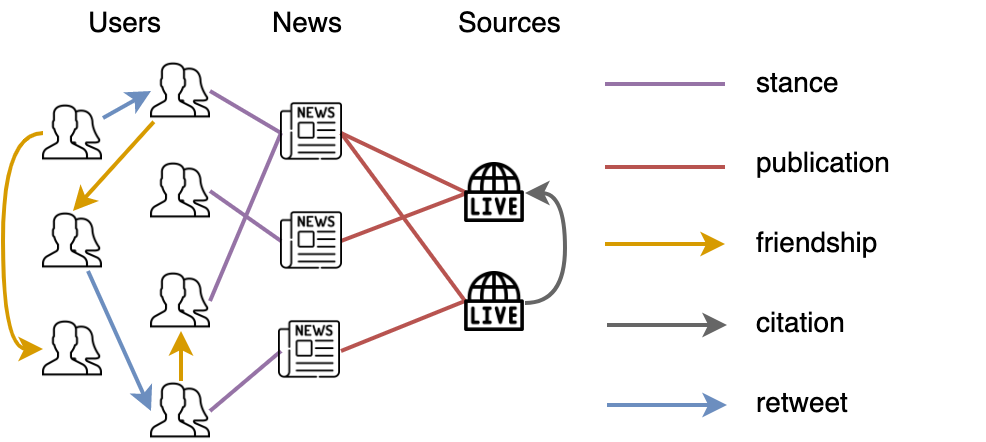
\includegraphics[scale=0.5]{social_graph_final.png}
\caption{Graph Representation of Social Context}
\label{fig:social_graph}
\end{figure}

\begin{table*}[t]
  \centering
  \tiny
  \begin{tabular}{|p{4cm}||p{1.5cm}|p{3cm}|p{5cm}|}
    \hline
    News title & Elapsed time - Total tweets  & Stance distribution - Support / Deny / Comment\_neutral / Comment\_negative / Report & Noticeable responses \\ \hline \hline
  Virginia Republican Wants Schools To Check Children's Genitals Before Using Bathroom & 3h - 38 & .00 / .03 / .03 / .16 / .78 & "DISGUSED SO TRASNPHOBIC", "FOR GODS SAKE  GET REAL GOP", "You cant make this up folks" \\ \cline{2-4}
  & (3h - 6h) - 21 & .00 / .10 / .05 / .05 / .80 & "Ok This cant be real", "WTF IS THIS BS", "Rediculous RT" \\ \cline{2-4}
  & $>$ 6h - 31 & .00 / .10 / .07 / .07 / .76 & "Cant make this shit up", "how is this real", "small government", "GOP Cray Cray  Occupy Democrats" \\ \hline
  \end{tabular}
  \caption{Temporal engagement of social users towards fake news}
  \label{table:temporal_engagement_fake}
\end{table*}

\begin{table*}[t]
  \centering
  \tiny
  \begin{tabular}{|p{4cm}||p{1.5cm}|p{3cm}|p{5cm}|}
    \hline
    News title & Elapsed time - Total tweets  & Stance distribution - Support / Deny / Comment\_neutral / Comment\_negative / Report & Noticeable responses \\ \hline \hline
  1,100,000 people have been killed by guns in the U.S.A. since John Lennon was shot and killed on December 8, 1980 & 3h - 9 & .56 / .00 / .00 / .00 / .44 & "\#StopGunViolence", "guns r the problem" \\ \cline{2-4}
  & $>$ 3h - 36 & .50 / .00 / .11 / .00 / .39 & "Some 1.15 million people have been killed by firearms in the United States since Lennon was gunned down", "\#StopGunViolence" \\ \hline
  \end{tabular}
  \caption{Temporal engagement of social users towards real news}
  \label{table:temporal_engagement_real}
\end{table*}

\section{Our Solution}
Social context of news dissemination is inherently representable as a heterogeneous graph whose nodes are the social entities and edges are the social interactions. A graph medium has several advantages over some existing Euclidean-based methods~\cite{ruchansky2017csi}~\cite{liu2018early} in terms of structural modeling capability for several phenomena like filtering bubbles of users or polarized network of news media. Network modelling also allows entities to exchange information, via heterogeneous edges, \textit{i.e}., 
% Min: use xx--yy not xx -- yy (GLOBAL).  I only changed here.
user--user relationship, source--source citations, heterogeneous edges, \textit{i.e}., user--news stance expression, source--news publication, and high order proximity, \textit{i.e}., between users who consistently support or deny certain sources, which are illustrated in  
%Such illustration is described in Figure~\ref{fig:social_graph}. 
Figure~\ref{fig:social_graph}.  
Previous attempts to learn such structure have employed spectral-based approaches ~\cite{shu2019beyond,gupta2012evaluating}, whose expensive matrix factorization does not account for higher order proximity, and whose representations are highly specific to the discussed task. Furthermore, there has been no in-depth analysis of the learned embeddings and their correlation to underlying communities, or whether the approach is feasible given a limited annotated news for supervised learning.

%Kaz: You can write like "Fake News Graph (FANG)" 
% Min: How about Factual News Graph, sounds more positive.
%We propose Fake News Graph or FANG, 
% Min: is it specific to fake news or more general?  If so the name should fit more specifically.
% Min: or say that FANG is an instance of the more general social context network 
We propose Fake News Graph (FANG), a graph learning framework for social context network in minimally supervised settings. 
%
FANG explores new information sources by looking at the news spreading pattern and temporality. FANG models the social actors --- \textit{i.e.}, news, sources, and users --- under a common medium that accounts for their interaction, and utilizes recent advancements in Graph Neural Network (GNN)~\cite{kipf2016semi,grover2016node2vec}. Given a joint representation space for social actors, we examine if the downstream node-level source factuality classification (SFC) can benefit from the embedding of the upstream fake news detection. FANG outperforms Euclidean baseline on fake news detection and achieves competitive performance given limited labels. We also analyze how the minimally supervised representations correlate with true labels, improving downstream analysis. The inductive nature of FANG is highly scalable in large graphs without concurrently storing all node features during training, and efficient in inference without re-processing the whole graph. Moreover, the prediction of FANG is easily explained thanks to the attention mechanism of its recurrent aggregator.

Our major contributions are summarized as follows:
\begin{enumerate}
    \item We provide a novel graph representation for the social context of news dissemination, which models all major social actors and interactions.
    \item We propose FANG, a novel graph learning framework that explores the unique structures of social context graph in minimally supervised settings.
    \item We conduct extensive experiments to assess the performance of FANG in fake news detection and its produced structural representations on downstream source factuality classification.
\end{enumerate}

%\section{Report Organization}
\section{Structure of Our Report}
%The structure of this report is organized as
This report is organized as follows: 
\begin{itemize}
    \item In Chapter 1, we introduce the problem of fake news, motivate the exploration of social context and present our solution of a novel graph representation and learning framework.
    \item In Chapter 2, we review the related literature in the domain of fake news detection and graph learning frameworks.
    \item In Chapter 3, we formalize the problems of representing social context and detecting fake news. We describe the proposed methodology to address the problems in details.
    \item In Chapter 4, we evaluate our proposed solution by analyzing the experimental results.
    \item In Chapter 5, we conclude the report with a discussion on future research directions.
\end{itemize}

\chapter{Related Work}
\label{ch:related}

We review the existing works on contextual fake news detection, which can be categorized by their approach to representation and learning of social context. Specifically, Euclidean approaches represents social context in the Euclidean space as a flat vector or matrix of real number. These methods typically learns a Euclidean transformation of social entity's features, \textit{i.e.,} the feature of social media who published and spread the news together with the news content itself, that best approximates the fake news prediction. The complexity of these transformation varies from the traditional non-deep models, \textit{i.e.,} Random Forest or Support Vector Machines (SVM)~\cite{castillo2011information,yang2012automatic} to deep networks including Long-short Term Memory~\cite{lstm1997hochreiter} that models engagement temporality~\cite{ruchansky2017csi}. However, given our formulation of social context as an heterogeneous network of social entities and their interaction, Euclidean representations are less expressive of structural information~\cite{bronstein2017geometric}. Although pioneering work employed individual attributes such as demographics, information preferences, social activeness, and structural features such as follower or friend counts~\cite{ma2015detect,shu2017fake}, they do not capture the user interaction landscape \textit{i.e.,} what kind of social figures they follow, which news topics they favor or oppose.

% specifically euclidean-based and network-based, which are more relevant to our research. We also discuss the recent advancement in Geometric Deep Learning framework, and how they can be applied to our social context graph. Here, we highlight the advantages and disadvantages of different methods, and motivate the choice of our solution.

% Even at group-level, user features are merely the aggregation of individual-level features like ``average number of users''~\cite{ma2015detect}. Such representations are relatively easy to construct and analyzed but completely lack the modelling capability for users from a common community. Furthermore, users can engage to a piece of news in different ways by expressing different stances or sentiments via various temporal patterns, which was not considered in these early works.

Having acknowledged such limitation, research have being exploring the non-Euclidean approach. Networks in which nodes constantly exchange and propagate information such as trust~\cite{kamvar2003eigentrust} or any auxiliary attributes~\cite{liao2018attributed} have been widely discussed. Recent works in detection falsehood has generalize the idea to social context by modelling an underlying user or news source network and dedicate a representation that captures an entity's structural features. CSI~\cite{ruchansky2017csi} used linear dimensionality reduction on user co-sharing adjacency matrix and combine it with the news engagement feature obtained from a recurrent neural network. TriFN~\cite{shu2019beyond}, which might seem similar to our proposal, neither differentiated user engagements in term of stance and temporal patterns, nor modeled source-source citation. Furthermore, such matrix decomposition approaches, including CSI~\cite{ruchansky2017csi}, are potential expensive in term of graph node counts and ineffective in modeling high-order proximity. Other works on citation source network~\cite{kulkarni2018multi}, propagation network~\cite{monti2019fake}, rumor detection~\cite{yuan2019jointly} utilized recent advances in graph neural network and multi-head attention attention to learn both local and global structural representation. Despite the incremental performance improvement in fake news detection, the authors neither considered a comprehensive social context graph or examined the representation learning of social entities in a minimally supervised setting. Table~\ref{table:literature_review} summarizes the comparison between the discussed works on representation learning frameworks of social context. The social entities and social interactions are (1) Users, (2) News, (3) Sources, (4) User -- user friendship, (5) User -- news engagement, (6) Source -- news publication, (7) Source -- citation.

\begin{table*}[t]
  \centering
  \tiny
  \begin{tabular}{|p{2.75cm}|p{3.5cm}|p{2.5cm}|p{1.25cm}|p{1.75cm}|p{1.75cm}|}
    \hline
    Approach & Category & Modeled social entities \& interactions & Temporality & Learning Framework & Structural Expressiveness \\ \hline \hline \cite{castillo2011information,ma2015detect,yang2012automatic} & Feature-based model & 1., 2. & No & Euclidean-based learning & No \\ \hline
    \cite{ruchansky2017csi} & Graph representation \& Euclidean learning & 1., 2., 4., 5. & Yes & Matrix factorization, Recurrent Neural Network & No \\ \hline
    \cite{shu2019beyond} & End-to-end Graph & 1., 2., 3., 4., 5., 6 & No & Matrix factorization & No \\ \hline
    \cite{kulkarni2018multi} & Graph representation \& Euclidean learning & 2., 3., 6., 7. & No & GNN, Deep Network  & No \\ \hline
    Monti (2019)~\cite{monti2019fake} & End-to-end Graph & 1., 2., 4., 5. & No & GNN & No \\ \hline
    \cite{yuan2019jointly} & End-to-end Graph & 1., 2., 5. & No & GNN, Multi-head attention & No \\ \hline \hline
    FANG (this work) & End2end Graph (supervised), Graph representation \& Euclidean learning (unsupervised) & 1., 2., 3., 4., 5., 6., 7. & Yes & GNN & Yes \\ \hline
    
  \end{tabular}
  \caption{Comparison between representation learning frameworks of social context}
  \label{table:literature_review}
\end{table*}
%Kaz: Did you define "GNN" before this paragraph/?

We also review the recent advancement of Graph Neural Network (GNN), the premise of our proposed framework.
GNNs have successfully generalize Deep Learning methods to model complex relationships and interdependency on graphs and manifolds. Graph Convolution Network (GCN) is one of the first proposal effectively approximate the parameters of convolutional filters~\cite{kipf2016semi}. However, spectral-based GCN requires substantial memory footprint to store the entire adjacency matrix, and is not easily adapted to heterogeneous graph where nodes and edges of different labels have different information propagation pattern. Spatial-based Graph Attention Network (GAT) addressed these limitations with batched aggregation strategy where information is selectively propagated from neighboring nodes~\cite{velivckovic2017graph}. Both GCN and GAT performs well on semi-supervised problem with moderate training data but deteriorates sharply given few training examples. Moreover, both are transductive approaches as they require inferred nodes to be present during training time, limiting the capability of online training. This is especially challenging in contextual fake new detection or general social network analysis as they structure is ever-evolving. With these caveats in mind, we built our work upon GraphSage that generates embeddings by sampling and aggregating features
from a node’s local neighborhood~\cite{Hamilton2017InductiveRL}. GraphSage provides great flexibility in defining the information propagation pattern with parameterized random walks and recurrent aggregator. Furthermore, GraphSage is highly suitable for representation learning with unsupervised node proximity loss and can address our problem of minimally supervised fake news detection.

%The comparison between the discussed works on representation learning frameworks of social context is summarized in Table~\ref{table:literature_review}


\chapter{Problem and Algorithm}
In this chapter, we first formulate the problem of fake news detection, and our research hypothesis. We then discuss the construction of social context graph, including feature extraction of each social entities and edge interaction labelling. We will describe the methodology of FANG in details as well as the intuition behind it.

\section{Fake News Detection from Social Context}
To ensure a consistent representation, let us first define social context, formulate the task of contextual fake news detection and formalize our research hypothesis. The fundamental entities and interactions of the social context $C$ are described as follows: 
\begin{enumerate}
    \item Let $A=\{a_1, a_2,...\}$ be the list of \textbf{news articles} that are being propagated through the social media. $a$ is defined by a feature vector $x_{a}$.
    \item Let $S=\{s_1, s_2,...\}$ be the list of \textbf{news sources} where each source $s_j$ has published at least one article in $A$. $s$ is defined by a feature vector $x_{s}$.
    \item Let $U=\{u_1, u_2,...\}$ be the list of \textbf{social users} where each user has engaged in spreading any article in $A$ or has a connection with any user in $U$. $u$ is defined by a feature vector $x_{u}$.
    \item Let $E=\{e_1, e_2,...\}$ be the list of interactions where each interaction $e=\{v_1, v_2, t, x_e\}$ describes an interaction between two entities $v_1, v_2\in A\cap S\cap U$ at time $t$, where $t$ can be absent in interactions that are time-insensitive. The interaction type of $e$ is defined as the label $x_{e}$.
\end{enumerate}
The characteristics of each interaction is further described in Table~\ref{table:social_interactions} and illustrated in Figure~\ref{fig:social_graph}.

\begin{table*}[t]
  \centering
  \tiny
  \begin{tabular}{|p{1.5cm}|p{2cm}|p{2.5cm}|p{5cm}|p{1cm}|}
    \hline
    Interaction & Linking entities & Linking type & Description & Time-sensitive \\ \hline \hline
    Followership & User-user & Unweighted, directed & Following/follower relationship on mainstream social media & No \\ \hline
    Citation & Source-source & Unweighted, directed & The percentage of reference hyperlink between one media source to another & No \\ \hline
    Publication & Source-news & Unweighted, undirected & The relationship between a media source and its published articles & Yes \\ \hline
    Stance & User-news & Multi-label, undirected & The perception of social users towards a news article & Yes \\ \hline
    Retweet & User-user & Unweighted, directed & The propagation of information from one user towards another & Yes \\ \hline 
  \end{tabular}
  \caption{Interactions in social context}
  \label{table:social_interactions}
\end{table*}

%Kaz: \textit{i.e}. => \textit{i.e}.*,*
Publication, stance and retweets are special types of interaction as it is not only characterized by its spatial features, \textit{i.e}., edge labels, source/destination nodes, but also by its temporal features, \textit{i.e}., when the interactions happen. Recent works have highlighted the importance of incorporating temporality in modeling social context engagement, not only in fake news detection~\cite{ruchansky2017csi}~\cite{ma2015detect}, but also in modeling online information dissemination~\cite{he2014predicting}. In this work, we are using six  stance labels, namely \textit{support}, \textit{deny}, \textit{negative\_comment}, \textit{neutral\_comment}, \textit{unrelated}, \textit{report}. Four of our stance labels, \textit{support}, \textit{deny}, \textit{comment}, \textit{unrelated} are consistent with the recent work on stance detection~\cite{mohtarami2018automatic}. Based on our observation of the distinguished sentiment of engagement towards fake and real news in Chapter~\ref{ch:introduction}, we classify \textit{comment} further into \textit{negative\_comment} and \textit{neutral\_comment}. We assign the ``report'' stance label to an user-news engagement when the user simply propagates the news article without expressing any opinion. Altogether, stances are used to characterize news articles by their perceived public opinions, as well as social users by their view on different journalism content. Table~\ref{table:stance_examples} shows examples for different stances.

\begin{table*}[t]
  \centering
  \tiny
  \begin{tabular}{|p{4cm}|p{7cm}|p{2cm}|}
  \hline
    News title & Tweet & Stance \\ \hline \hline
  US Representatives Agree To Illicit UN Gun Control Plans & More proof we should pull out of the UN and throw them out of the US Pot us Real Donald Trump US Representative & support \\ \cline{2-3}
  & This can't be right & deny \\ \cline{2-3}
  & Oh my giddy aunt & neutral\_comment \\ \hline
  Pence Michelle Obama Is The Most Vulgar First Lady We've Ever Had & How dare you sir that's our First Lady respect Pence Michelle Obama Is The Most Vulgar First Lady We've Ever Had & negative\_comment \\ \cline{2-3}
  & RT Janice GW Pence Michelle Obama Is The Most Vulgar First Lady We've Ever Had USA Newsflash & report \\ \cline{2-3}
  & Lawrence run with this PLEASE & unrelated \\ \hline
  \end{tabular}
  \caption{Examples of user stances towards news articles}
  \label{table:stance_examples}
\end{table*}

We refer to the definition of general Fake News Detection by Kaishu~\cite{shu2017fake} and formally define the task of context-based Fake News Detection.
\begin{definition}{\textit{Context-Based Fake News Detection}}: Given a social context $C(A,S,U,E)$ constructed from news articles $A$, news sources $S$, social users $U$, and social engagements $E$,
%Kaz: Can you rephrase "Context-based Fake News Detection" to "Context-based FND" as FND is used in the previous part. 
%Hoang: Thank you, I have rephrased.
Context-based Fake News Detection is defined as the binary classification task of predicting whether a news article $a\in A$ is fake or not, \textit{i.e}.,  $F_C : a \rightarrow \{0,1\}$ such that,
\[  F_C(a) = \left\{
\begin{array}{ll}
      0 & \textrm{if } a \textrm{ is a fake article} \\
      1 & \textrm{otherwise} \\
\end{array} 
\right. \]
\end{definition}
Context-based Fake News Detection is considered a semi-supervised learning problem where we train our classifier on the partially labelled articles to approximate $F_C$ and predict whether the unlabeled articles are fake or not.
\begin{hypothesis}Given a social context $C(A,S,U,E)$, we hypothesize that our graph representation and learning framework, \textit{i.e}., FANG, improve the structural features of social actors $A,S,U$, resulting in more accurate fake news detection.
\end{hypothesis}

\section{Graph Construction from Social Context}
\label{sec:graph_construction}
In this section, 
%Kaz: Rephrased the following phrase. You can use "detail"  as a verb. 
%we describe details 
we detail our social context graph construction. We specify the selected features for each social entities, \textit{i.e}., $x_a$, $x_s$, $x_u$, and how we obtain the labels for each social interaction, \textit{i.e}., $x_e$.

\textbf{News Articles}: News content is a major component in detecting the authenticity of the news itself. Textual~\cite{castillo2011information}~\cite{yang2012automatic}~\cite{shu2019beyond}~\cite{popat2018credeye} and visual~\cite{wang2018eann}~\cite{khattar2019mvae} have been widely used to model news article contents, either by feature extraction, unsupervised semantics encoding, or learned representation. In this work, we are looking at unsupervised semantics encoding as it is relatively efficient to construct and optimize. We are aware of non-end-to-end limitation and would like to leave this as an open research question.

In the scope of this report, we consider only textual features. For each article $a\in A$, we constructed the tf-idf~\cite{sparck2004idf} vector $v^t_a$ from text body in the article. We increase the semantics expressiveness of token-based representation by weighting them with pre-trained word embeddings obtained from GloVe~\cite{pennington2014glove} to obtain $v^s_a$. The news article feature vector $x_a$ is created by concatenating $v^t_a$ and $v^s_a$.

\textbf{News Sources}: Characteristics of media sources that publishes the questionable news have been widely adopted as a essential indicator of the news trustworthy~\cite{baly2018predicting}~\cite{kulkarni2018multi}. Commonly utilized features include journalism topics, lexicon-derived bias, url structure and social network trace~\cite{baly2018predicting}. This report focuses mainly on characterizing media sources by their reporting textual content. For each source $s$, similar to article representations, we constructed the source feature vector $x_s$ 
%Kaz: You can just describe "tf-idf vector" not "a bag-of-word tf-idf vector" as we often use a "bag-of-word vector". 
as the concatenation of a bag-of-word tf-idf vector $v^t_s$ and a semantics-sensitive vector $v^s_s$ derive from the ``homepage'' and ``about-us'' directory. A portion of fake news spreading websites give a ``disclaimer'' of being a satirical or sarcastic media in the their ``about-us'' --- a helpful signal for the journalism quality. 

\textbf{Social Users}: Online users have been studied extensively as the major propagator of fake news and rumors in social media. As discussed in chapter~\ref{ch:related}, previous work~\cite{castillo2011information}~\cite{yang2012automatic} utilized attributes  such  as  demographics,  information  preferences,  social activeness, and network structure such as follower or friend counts. A recent work by Kai Shu~\cite{shu2019role} conducted a feature analysis on user profile and pointed out the importance of signals derived from profile description and timeline content. A text description such as "American mom fed up with anti american leftists and corruption. I believe in US constitution, free enterprise, strong military and Donald Trump \#maga" strongly indicates the user political bias and suggest the tendency to promote certain narratives. We calculate the user vector $x_u$ as the concatenation of a pair of tf-idf vector $v^t_u$ and semantics vector $v^s_u$ derived from the user profile text description.

\textbf{Social interactions}: For every social actor pairs $(v_i, v_j)\in A\cap S\cap U$, we add an edge $e=\{v_i, v_j, t, x_e\}$ to the list of social interactions $E$ if they interact via interaction type $x_e$. Specifically, for followership, we examine if user $u_i$ follows user $u_j$ on social media; for publication, we examine if news $a_i$ was published by source $s_j$; for retweet, we examine if user $u_i$ has ever retweeted user $u_j$; for citation, we examine if the homepage of source $s_i$ contains any hyperlink to source $s_j$. In the case of time-sensitive interactions, \textit{i.e}. \textit{publication}, \textit{retweet} and \textit{stance}, we record their relative timestamp with respect to the article's earliest publication time. 

\textbf{Stance detection}: The task of obtaining a the point of view of a source text towards a target text is commonly known as \textit{stance detection}~\cite{Kk2020StanceDA}. In our context of fake news detection, the target is the title of the questionable news while the source text is the user comments on the when they decide to retweet or reply it. Popular stance detection dataset either do not explicitly describe the target text~\cite{derczynski-etal-2017-semeval}, have a limited number of targets~\cite{sobhani-etal-2017-dataset,mohammad-etal-2016-semeval} or formulate the source and target text differently (Fake News Challenge~\footnote{\scriptsize{\url{http://www.fakenewschallenge.org/}}}). 

As one of the pioneering work, we have constructed a novel dataset for stance detection between tweets and news. We use this dataset to supervisedly train our classifier for ``support'' and ``deny'' stances. This dataset contains 2527 labeled source -- target sentence pairs from 29 news events. For each event with a reference headline, annotator are given a list of related headlines and tweets. The annotation task is to label whether each related headline and tweet supports or denies the claim made by the reference headline. Besides the reference headline -- related headline or headline -- related tweet sentence pairs, we also made a second order inference for related headline -- related tweet sentence pairs. If such pair expressed a similar stance towards the reference headline, the inferred stance for related headline -- related tweet would be ``support'', and vice versa. An example annotation is shown in Table~\ref{table:stance_annotation}, while the dataset statistics are presented in Table~\ref{table:stance_statistics}. The inter annotator agreement Cohen's Kappa score is 0.7776, indicating a substantial agreement.

\begin{table}[t]
  \centering
  \small
  \begin{tabular}{|p{2cm}|p{7.25cm}|p{2.75cm}|p{2cm}|}
  \hline
    Event ID & Text & Type & Annotated Stance \\ \hline \hline
  greta-pay & Greta Thunberg tops annual list of highest-paid Activists! & reference headline & - \\ \hline
  greta-pay & Greta Thunberg is the ‘Highest Paid Activist’ & related headline & support \\ \hline
  greta-pay & No, Greta Thunberg not highest paid activist & related headline & deny \\ \hline
  greta-pay & Can't speak for the rest of 'em, but as far as I know, Greta's just a schoolgirl and has no source of income. & related tweet & deny \\ \hline
  greta-pay & The cover describes Greta Thunberg to be the highest paid activist in the world & related tweet & support \\ \hline
  greta-pay & Can't speak for the rest of 'em, but as far as I know, Greta's just a schoolgirl and has no source of income. & related tweet & deny \\ \hline
  \end{tabular}
  \caption{An example in the stance-annotated dataset}
  \label{table:stance_annotation}
\end{table}

\begin{table}[t]
  \centering
  \small
  \begin{tabular}{|p{2cm}|p{2cm}|p{2cm}|p{2cm}|p{2cm}|}
  \hline
    & \# News & \# Samples & \# Supports & \# Denies \\ \hline \hline
  Train & 29 & 2089 & 931 & 1158 \\ \hline
  Test & 2 & 438 & 207 & 231 \\ \hline
  \end{tabular}
  \caption{An example in the stance-annotated dataset}
  \label{table:stance_statistics}
\end{table}

To choose the best stance classifier, we fine-tune pre-trained Language Models built upon large-scale transformers like BERT on our dataset. These are the models that have achieved state-of-the-art performance on many Natural Language Understanding tasks~\cite{wang-etal-2018-glue}. Roberta~\cite{liu2019roberta} is the best performing model in test set with 0.8857 \textit{Accuracy}, 0.8379 \textit{Macro $F_1$}, 0.8365 \textit{Precision}, 0.8395 \textit{Recall} and is chosen as our stance classifier. The stance prediction of a user -- article engagement $e$ is given as $stance(e)$.

\section{FANG}
\label{sec:fang}

\begin{figure}[t]
\centering
\includegraphics[scale=0.6]{fang.png}
\caption{Overview of FANG famework}
\label{fig:fang_overview}
\end{figure}

In this section, we describe our FAke News Graph learning framework or FANG learning framework on the social context graph described in Section~\ref{sec:graph_construction}. The overview of FANG is described in Figure~\ref{fig:fang_overview}. As discussed, FANG's motivation is not only to improve the performance of contextual fake news detection, but also to improve the representation learning quality. That is, while optimizing for the fake news detection objective, FANG also learns meaningful representations of social entities being highly generalizable to downstream tasks. This is achieved by optimizing for three concurrent objective: unsupervised \textit{Proximity Loss}, self-supervised \textit{Stance Loss}, and supervised \textit{Fake News Detection}.

\textbf{GraphSage Representation Learning}. Before describing the details of each learning objective, we first discuss how FANG derived the representation of each social entities. Previous representation learning framework on graph including Deep Walk~\cite{perozzi2014deepwalk} or node2vec~\cite{grover2016node2vec} computes a node embedding by sampling its neighbor and optimizing for the proximity loss. However, these methods are most effective when the node auxiliary features are not available or complete, therefore separately optimize for each entity structural representation. A recent graph neural network, GraphSage~\cite{Hamilton2017InductiveRL}, addressed this limitation by leveraging node auxiliary features jointly with proximity sampling in representation learning. Let $GraphSage(.)$ be GraphSage's node encoding function, we obtained the structural representation $z_u\in \mathbb{R}^d$ of node $u$ as $z_u=GraphSage(u)$.

\textbf{Unsupervised Proximity Loss}. We derive the Proximity Loss from our hypothesis that closely connected social entities often behave similarly. This hypothesis is motivated by the ``echo chamber'' phenomenon, where social entities tend to interact with other entities of common interest to reinforce and promote their narrative. The ``echo chamber'' phenomenon includes inter-cited media sources publishing news of similar content or factuality, and social friends expressing similar stance towards a piece of news or news articles of similar content. Therefore, FANG should assign such nearby entities a set of closed vectors in the embedding space. We also hypothesize that loosely connected social entities often behave differently. We observed that social entities are highly polarized, especially on left-right politics -- the topic most bombarded by false information~\cite{boxell2017internet}. FANG should enforce the representations of these disparate entities to be highly distinct.

The social interactions that most define the above characteristics are user -- user friendship, source -- source citation and news -- source publication. As these interactions are either between sources and news or between news, we divide the social context graph into 2 sub-graphs, \textit{i.e.} news -- source sub-graph and user sub-graph. Within each sub-graph $G$ we formulate the Proximity Loss function as
\begin{equation}\label{eq:proximity_loss}
    \mathcal{L}_{proximity} =  - \sum_{u\in G} \sum_{u_p\in P_u} log(\sigma(z_u^\top z_{u_p})) + Q \cdot \sum_{u_n\in N_u} log(\sigma(-z_u^\top z_{u_n}))
\end{equation}
where $z_u\in \mathbb{R}^d$ is the representation of entity $u$, $P_u$ is the set of nearby nodes or \textit{positive set} of $u$, and $N_u$ is the set of disparate nodes or \textit{negative set} of $u$. $P_u$ is obtained my fixed length Random Walk, while $N_u$ is obtained by negative sampling. Each $u_n\in N_u$ is sampled with the discrete probability density function $\forall v\in G\setminus P_u, P(u_n=v) = \frac{x_u^\top x_v}{Z}$ where $x_u$ and $x_v$ are the feature vectors of entity $u$ and $v$, and $Z$ is the probabilistic normalization factor. In other word, we choose the negative samples of an entity $u$ based on the feature distance between $u$ and the candidate sample $v$ which is not in the positive samples. By minimizing the proximity loss described in Equation~\ref{eq:proximity_loss}, we effectively force the representations of closed entities to be similar and the representations of disparate entities to be distinct.

\textbf{Self-supervised Stance Loss}.
For the user -- news interaction in terms of stance, we also put forward a analogous hypothesis. A user and news article pairs who express a stance should have their representation closed in that stance space. For each stance $c$, we first learn a user projection function $F^u_c(u) = A^u_c z_u$ and a news article projection function $F^a_c(a) = A^a_c z_a$ that maps a node representation of $\mathbb{R}^d$ to representation in stance $c$ space of $\mathbb{R}^{d_c}$. Given a user $u$ and a news article $a$, we compute their similarity score in stance $c$ space as $F_c(u)^T F_c(a)$. If $u$ actually expresses stance $c$ towards $a$, we would like to maximize this similarity score, and vice versa, minimize this similarity score otherwise. We interpret this objective as a stance classification objective which can be optimized by the following Stance Loss.
\begin{equation}
    \mathcal{L}_{stance} = -\sum_{u,a,c} y_{u,a,c} log(f(u,a,c))
\end{equation}
where $f(u,a,c)$ is defined as
\begin{equation}
    f(u,a,c) = F_c(u)^T F_c(a)
\end{equation}
and
\[  y_{u,a,c} = \left\{
\begin{array}{ll}
      1 & \textrm{if } u \textrm{ expresses stance } c \textrm{ over } a \\
      0 & \textrm{otherwise} \\
\end{array} 
\right. \]
Note that the stance label $c$ of an engagement $e$ between user $u$ and article $a$ is defined as $stance(e)$ using the stance classifier described in Section~\ref{sec:graph_construction}. By optimizing for the above stance edge classification objective, we effectively force the representations of an engaged user -- news article via a stance to be closed in that stance space.

\textbf{Supervised Fake News Loss}. We directly optimize for the main learning objective of fake news detection via the supervised Fake News Loss. This can be formulated as learning an aggregation function $F(a, s, U)$ that maps a questionable news $a$, its source $s$ and its engaged users $U$ to a real number in $[0, 1]$, indicating the probability of $a$ being trustworthy. As observed in Chaper~\ref{ch:introduction}, we hypothesize that there are distinctive temporal patterns between false and genuine information. Therefore, the aggregating model, \textit{i.e.} the aggregator, has to be time-sensitive. Recurrent Neural Networks fulfilled such a requirement where the Bidirectional Long-short Term Memory (BiLSTM) can capture a long-term dependency in information sequence in forward and backward directions~\cite{lstm1997hochreiter}. On top of the vanilla BiLSTM, we also incorporate an attention mechanism that focus on essential engagement during the encoding process. Attention mechanism is not only expected to improve our model quality but also its explanability~\cite{luong2015effective,vaswani2017attention}. By examining the model's attention, we would know which Twitter profiles influenced its decision, therefore leverage not only the machine but also human analytic capability. Our proposed LSTM's input is a user -- article engagement sequence $\{e_1, e_2,\cdots,e_{|U|}\}$. Let $meta(e_i)\in \mathbb{R}^l=(time(e_i),stance(e_i))$ be the concatenation $e_i$ stance and meta. Each engagement $e_i$ has its representation $x_{e_i}$ following form:

\begin{equation}
    \boldsymbol{x}_{e_i} = (\boldsymbol{z}_{U_i}, meta(e_i))
\end{equation}
where $\boldsymbol{z_{U_i}}=GraphSage(U_i)$, $time(e_i)$ and $stance(e_i)$ are the time since published and stance of engagement $e_i$ respectively. 

A BiLSTM encodes the engagement sequence and outputs two sequence of hidden states: a forward sequence,
$H^f={\boldsymbol{h}^f_1, \boldsymbol{h}^f_2,\ldots,
  \boldsymbol{h}^f_n}$ that starts from the beginning of the engagement sequence; and
a backward sequence, $H^b={\boldsymbol{h}^b_1,
  \boldsymbol{h}^b_2,\ldots, \boldsymbol{h}^b_n}$ that starts from the
end of the engagement sequence. For many sequence encoding tasks, knowing both past
(left) and future (right) contexts has proven to be effective~\cite{dyer2015transition}. The states $\boldsymbol{h}^f_i$ and $\boldsymbol{h}^b_j$ in
the forward and backward sequences are computed as:
\begin{eqnarray}
  \boldsymbol{h}^f_i=LSTM(\boldsymbol{h}^f_{i-1}, \boldsymbol{x_{e_i}}),
  \hspace{1mm}\boldsymbol{h}^b_j=LSTM(\boldsymbol{h}^b_{j+1}, \boldsymbol{x_{e_j}}), \nonumber 
\end{eqnarray}
where $e$ is the number of encoder units, and $\boldsymbol{h}^f_i, \boldsymbol{h}^b_j\in \mathbb{R}^e$ are the $i$th and $j$th hidden state vector of the forward ($f$) and backward ($b$) sequence. Let $w_i$ be the attention weight paid by our BiLSTM encoder to the forward ($\boldsymbol{h}^f_i$) and backward ($\boldsymbol{h}^b_i$) hidden states. This attention should be derived from the similarity of the hidden state and the news features, \textit{i.e.} how relevant the engaging users are to the discussed content, and the particular time and stance of the engagement. Therefore, we formulate the attention weight $w_i$ as:
\begin{equation}
    w_i = \frac{exp(\boldsymbol{z}_a \mathbf{A}^e  \boldsymbol{h}_i + meta(e_i) \mathbf{A}^m)}{\sum^n_{j=1}exp(\boldsymbol{z}_a \mathbf{A}^e \boldsymbol{h}_j + meta(e_j) \mathbf{A}^m)}.
\end{equation}
Let $l$, $d$, $e$ are the meta dimension, structural embedding dimension and encoder dimension, $\mathbf{A}^e\in \mathbb{R}^{d\times e}$ and $\mathbf{A}^m\in \mathbb{R}^{l\times 1}$ are the optimizable projection matrices shared across all engagements. $w_i$ is then used to compute forward and backward weighted feature vectors:
\begin{eqnarray}\label{eq:w_sum}
  \boldsymbol{h}^f=\sum^n_i w_i \boldsymbol{h}^f_i, 
  \quad\boldsymbol{h}^b=\sum^n_i w_i \boldsymbol{h}^b_i. 
\end{eqnarray}
We concatenate the forward and backward vectors to obtain a single representation engagement $\boldsymbol{r}_a$ for article $a$, following previous bi-directional LSTM practice~\cite{ma2016end}.

To predict whether article $a$ is false, we use a combination of the its structural representation $\boldsymbol{z}_a$, its engagement representation $\boldsymbol{r}_a$ and its source $s$'s structural representation $\boldsymbol{z}_s$. The article's contextual representation is obtained as the combination of all these features:
\begin{equation}
    \boldsymbol{v}_a = (\boldsymbol{z}_a, \boldsymbol{r}_a, \boldsymbol{z}_s)
\end{equation}
This contextual representation is input into a fully connected layer whose outputs are computed as:
\begin{equation}
    o_a = \mathbf{W}v_a+b
\end{equation}
where $\boldsymbol{W}\in \mathbb{R}^{2e\times 1}$ and $b\in \mathbb{R}$ are weights and biases of the layer. The output value $o_a \in \mathbb{R}$
is finally passed through a sigmoid activation function $\sigma(\cdot)$, and trained using cross-entropy Fake News Loss $\mathcal{L}_{news}$ defined as follows:   
\begin{equation}
    \mathcal{L}_{news}=\frac{1}{T}\sum_a\{{y}_{a} \cdot log(\sigma({o}_{a}))+(1-{y}_{a})\cdot log(1-\sigma({o}_{a}))\}
\end{equation}
where $y_{a}=0$ if $a$ is a fake article and $1$ otherwise.

\textbf{End-to-end Total Loss}. We define the Total Loss as the sum of three loss, namely Proximity Loss, Stance Loss and Fake News Loss.
\begin{equation}
    \mathcal{L}_{total} = \mathcal{L}_{proximity} + \mathcal{L}_{stance} + \mathcal{L}_{news}
\end{equation}
The loss function is differentiable, thus trainable with the Adam optimizer~\cite{kingma2015adam}. 

\chapter{Results}
In this section, we conducted experiments to evaluate the effectiveness of our proposed Graph Representation and Learning Framework. We will find answers to the following research questions (RQs):
\begin{itemize}
    \item RQ1: Does FANG work better than content-only models, contextual Euclidean models and contextual graph models?
    \item RQ2: Does FANG work well with limited training data?
    \item RQ3: What is the rationale behind temporality awareness of our model?
    \item RQ4: How effective is FANG's representation learning
    \begin{itemize}
        \item RQ4a: via intrinsic evaluation?
        \item RQ4b: via extrinsic evaluation?
    \end{itemize}
\end{itemize}

\section{Dataset and Experiment Settings}
We conducted our experiments on Twitter dataset collected by related-work in rumor classification~\cite{ma2016detecting} and fake news detection~\cite{shu2018fakenewsnet}. For each article, its source and the list of users and their tweets discussing it were collected. Our dataset includes Twitter profile description and the list of Twitter profiles they follow. We crawl additional data of media sources, including the content of their homepage and ``about-us'' page, together with their frequently cited sources by collecting the hyperlink references in their homepage. The source truths of the articles, \textit{i.e.} whether are false or genuine, are based on two fact-checking websites -- Snopes~\footnote{\url{https://www.snopes.com}} and Politifact\footnote{\url{https://www.politifact.com}}. The statistics of our dataset are described in Table~\ref{table:dataset_statistics}.

\begin{table}[ht]
    \centering
    \begin{tabular}{l | l} \hline
        \# Fake News & 150 \\
        \# Real News & 151 \\
        \# Sources & 199 \\
        \# Users & 199 \\ \hline
        Avg. citation / source & 5.11 \\
        Avg. publication / source & 1.51 \\
        Avg. friendship / user & 85.78 \\
        Avg. support / news & 99.14 \\
        Avg. deny / news & 13.44 \\
        Avg. report / news & 70.25 \\
        Avg. engagement / news & 182.84 \\ \hline
    \end{tabular}
    \caption{Some statistics on our dataset.}
    \label{table:dataset_statistics}
\end{table}

\section{Macroscopic Analysis.}\label{sec:macroscopic}
To address RQ1, we benchmark FANG performance in Fake News Detection against a content-only baseline, a Euclidean contextual baseline and another Graph Learning baseline. For the first confirmation on superiority over the content-only model, we train a Support Vector Machine model on Tf-idf feature vectors constructed from news content (Section~\ref{sec:graph_construction}). For the second confirmation on superiority over Euclidean models, we choose CSI~\cite{ruchansky2017csi}, a fundamental yet effective recurrent encoder that aggregate the user features, news content and user -- news engagements. We supplement the original implementation with source features by concatenating the user overall score, the article representation with our formulated source description to obtain the result vector in the Integrate module. We also verify the importance of temporality by conducting the experiments on two variants for both CSI and FANG: (1) i-CSI and i-FANG where we do not include $time(e)$ in the engagement $e$'s representation $\boldsymbol{x_{e_i}}$, and (2) CSI and FANG where we include $time(e)$. For the third confirmation on the superiority over other Graph Learning frameworks, we choose Graph Convolutional Network~\cite{kipf2016semi}. In consistent with the original paper, we define $X\in \mathbb{R}^{N\times d_1}$ to be the input node feature matrix where $X^{(i)}\in \mathbb{R}^{d_1}$ is the feature vector of $i$th social actor defined in section~\ref{sec:graph_construction}. Let $d_l$ be the size of any node hidden representation obtained at the $l$th layer of GCN. We define the convolution operation in our graph consisting of multi-label edges as
\begin{equation}
    H_{l+1} = \parallel^{K}_{k=1}(\tilde{D}^{-\frac{1}{2}}\tilde{M}_k\tilde{D}^{-\frac{1}{2}}H_l\Theta_l)
\end{equation}
where $H_l\in \mathbb{R}^{N\times d_l}$ is the hidden representation matrix of social actors at $l$th layer, $\parallel$ is the concatenation operation, $K$ is the number of relations, $\Theta\in\mathbb{R}^{d_l\times d_{l+1}}$ is the matrix of optimizable weights at $l$th layer, and $\tilde{D}^{-\frac{1}{2}}\tilde{M}_k\tilde{D}^{-\frac{1}{2}}$ is the computation to obtain normalized graph Laplacian matrix. Notice that $H_1=X$ is the input feature matrix. After L layers, we obtain the output vector as the final hidden representation of each article $a$, or $\boldsymbol{o_a}=H^{(\bar{a})}_L$ where $\bar{a}$ is the index of $a$. $\boldsymbol{o_a}$ is passed through a softmax activation function $\sigma$, and all learnable weights are trained using cross-entropy loss as defined by $\mathcal{L}$:
\begin{equation}\label{eq:overall_loss}
    \mathcal{L}=\frac{1}{|A_c|}\sum^{A_c}_{a}\boldsymbol{y}_{a} \cdot log(\sigma(\boldsymbol{o}_{a}))+(1-\boldsymbol{y}_{a})\cdot log(1-\sigma(\boldsymbol{o}_{a}))
\end{equation}

We use $F_1$ score -- the harmonic mean of Precision and Recall to evaluate all models' performance in Fake News Detection. The macroscopic results are presented in Table~\ref{table:macroscopic}

\begin{table}[ht]
    \centering
    \begin{tabular}{c| c c c| c} \hline
        Systems & Context-aware & Temporality-aware & Graph-based & $F_1$ score \\ \hline
        Feature-only SVM & & & & 0.6785 \\
        i-CSI & \checkmark & & &  0.7529 \\
        CSI & \checkmark & \checkmark & & 0.8055 \\ 
        GCN & \checkmark & & \checkmark & 0.8090 \\
        i-FANG & \checkmark & & \checkmark & 0.8889 \\ \hline
        FANG & \checkmark & \checkmark & \checkmark & 0.9519 \\ \hline
    \end{tabular}
    \caption{Performance of FANG versus baseline models in fake news detection measured by $F_1$ score.}
    \label{table:macroscopic}
\end{table}

\section{Limited Training Data.}
To address RQ2, we conducted the experiments described in Section~\ref{sec:macroscopic} given varying training data availability. These experiments confirm our model's consistent absolute performance and relative improvement over baseline models given both limited and sufficient data. The experiment results are represented in Table~\ref{table:limited_data} and visualized in Figure~\ref{fig:limited_data}.

\begin{table}[ht]
    \centering
    \begin{tabular}{l | l l l l l} \hline
        Systems & $F_1@0.9$ & $F_1@0.7$ & $F_1@0.5$ & $F_1@0.4$ & $F_1@0.1$ \\ \hline
        CSI & 0.8055 & 0.7546 & 0.6851 & 0.7443 & 0.743 \\
        GCN & 0.809 & 0.6523 & 0.6407 & 0.6866 & 0.6123 \\ \hline
        FANG & 0.9519 & 0.8218 & 0.801 & 0.8366 & 0.8274 \\ \hline
    \end{tabular}
    \caption{Performance of FANG against baselines given varying training availability in terms of $F_1$ score.}
    \label{table:limited_data}
\end{table}

\begin{figure}[ht]
\centering
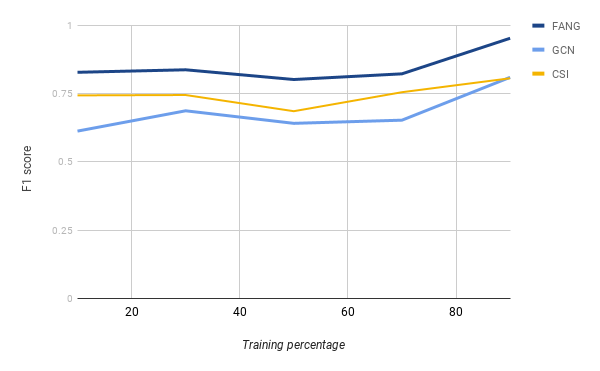
\includegraphics[scale=0.7]{limited_data.png}
\caption{Experiment result plot}
\label{fig:limited_data}
\end{figure}

\section{Temporality study.} To address RQ3 and verify that our model makes its decision based on the distinctive temporal patterns between fake and real news, we examine FANG's attention. We accumulate the attention weights produced by FANG within each time window and compare them across time windows. Figure~\ref{fig:fang_attention} describes such attention distribution over time with regards to fake and real news.

\begin{figure}[ht]
\centering
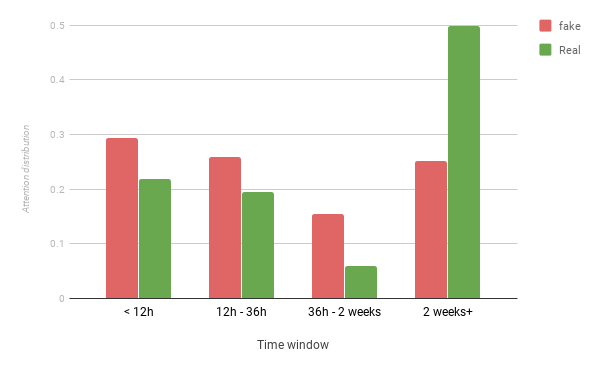
\includegraphics[scale=0.7]{fang_attention.png}
\caption{FANG's attention distribution across time windows with regards to fake and real news}
\label{fig:fang_attention}
\end{figure}

\section{Representation learning.}
We verify the improved quality of our representations in both intrinsic and extrinsic evaluations, hence address RQ4. 

\begin{figure}[ht]
\centering
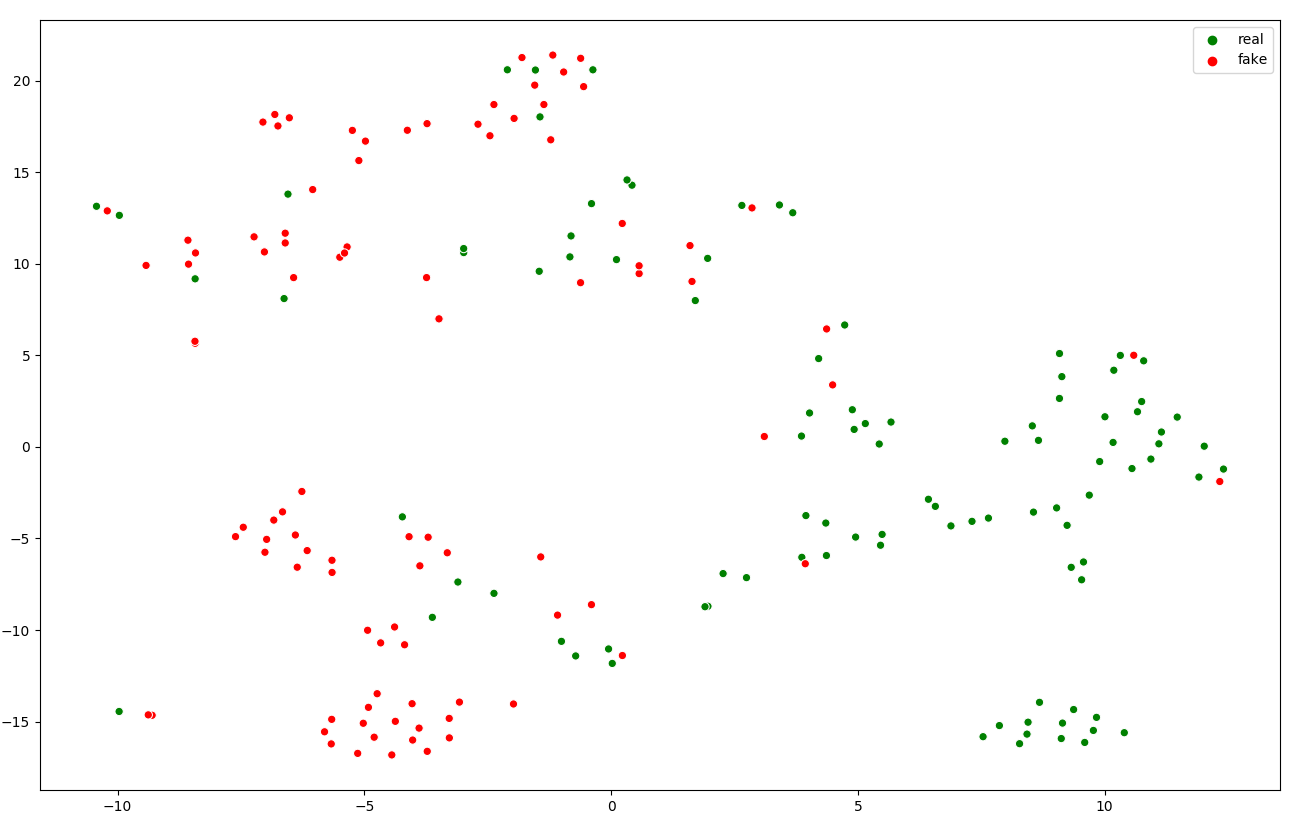
\includegraphics[scale=0.23]{fang_tsne.png}
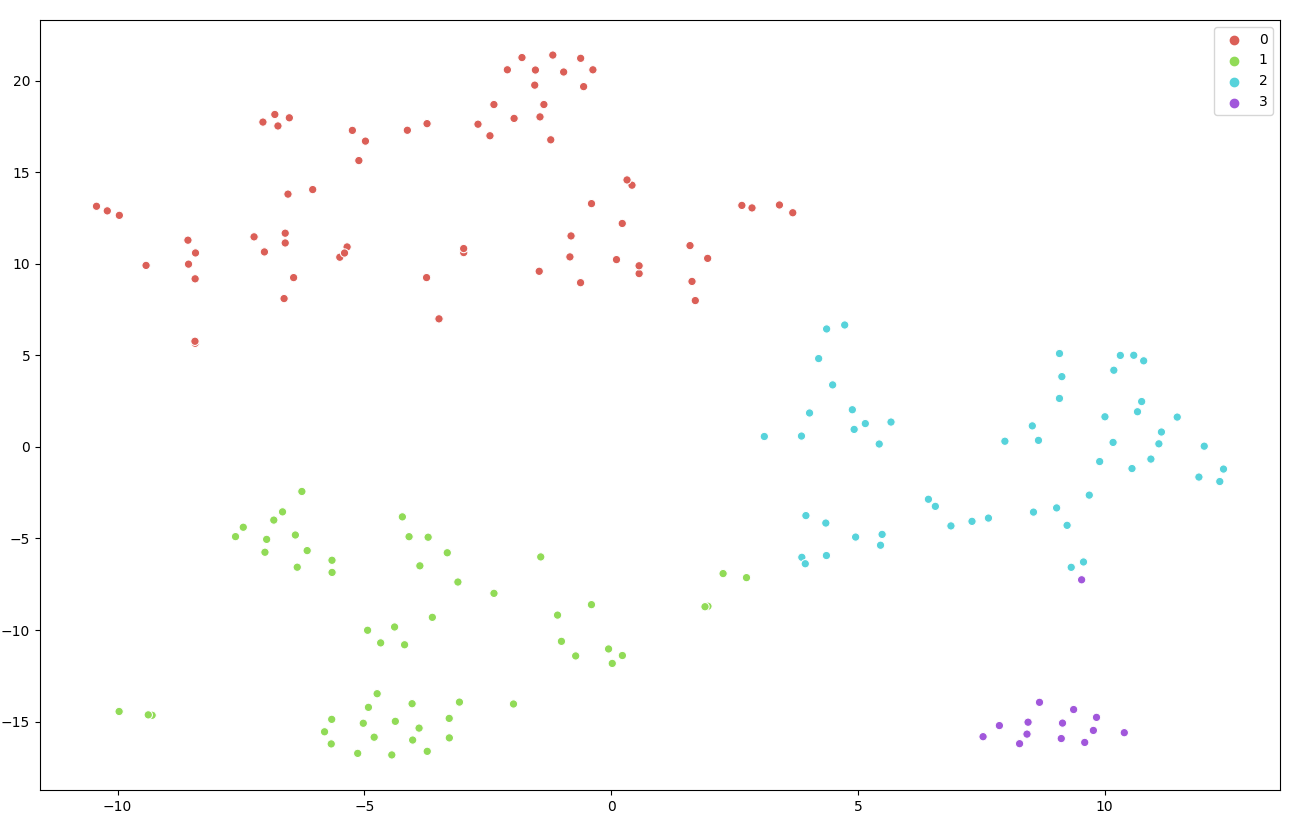
\includegraphics[scale=0.23]{fang_clusters.png}\\
\caption{2D t-SNE plot of FANG's representations with factuality news labels (left) and Mean shift clustering labels (right)}
\label{fig:fang_rep}
\end{figure}

\begin{figure}[ht]
\centering
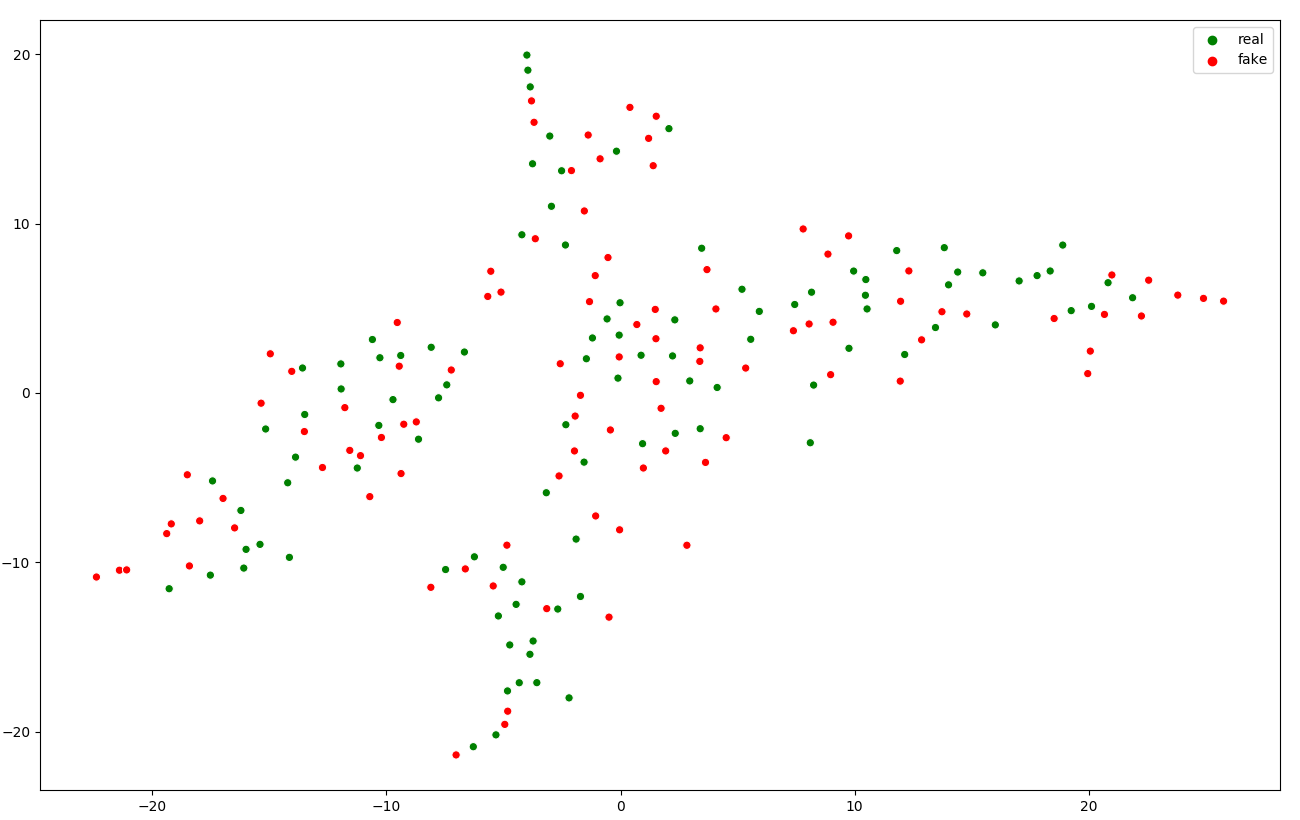
\includegraphics[scale=0.23]{gcn_tsne.png}
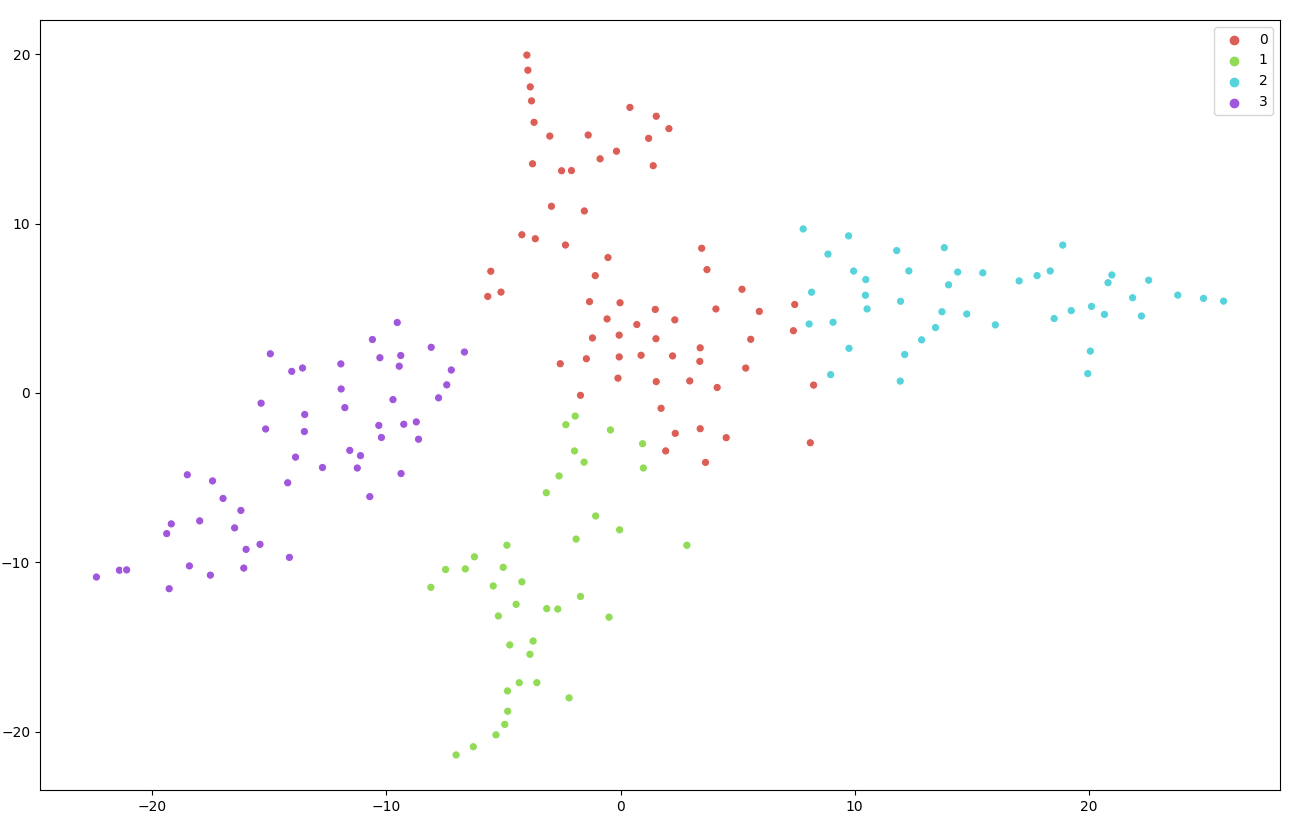
\includegraphics[scale=0.23]{gcn_clusters.png}\\
\caption{2D t-SNE plot of GCN's representations with factuality news labels (left) and Mean shift clustering labels (right)}
\label{fig:gcn_rep}
\end{figure}

In the intrinsic evaluation, we verify how generalizable the minimally supervised news representations are in the intrinsic fake news detection task. In specific, we first optimize FANG on 10\% training data to obtain all news representations. We then cluster these representations using Mean shift~\cite{Comaniciu2002meanshift}, an unsupervised clustering algorithm, and measure the homogeneity score -- the extent to which clusters contain a single class. The higher the homogeneity score is, the more likely news articles of similar factuality labels, \textit{i.e.} fake or real, are closed to each other and the higher quality their representations are. We visualize FANG's representations in 2-dimension with factuality labels (Figure~\ref{fig:fang_rep}'s left) and Mean shift clustering labels (Figure~\ref{fig:fang_rep}'s right). We also provide GCN's representations, which is a fully supervised approach in Figure~\ref{fig:gcn_rep}, to benchmark FANG's representation quality against.

In the extrinsic evaluation, we verify how generalizable the sufficiently supervised source representation are in the extrinsic source factuality classification task. In specific, we first optimize FANG on 90\% training data to obtain all any source $s$'s representation as $z_s=GraphSage(s)$. We then obtain source $s$'s total representation $r_s$ as

\begin{equation}
    v_s=(z_s,x_s,\sum_{a\in publish(s)}x_a)
\end{equation}
where $x_s$ is source $s$'s content representation, $publish(s)$ is the list of all articles published by $s$ and $x_a$ are their content representations. We propose two baseline representations that does not consider source $s$ content, $v^{\prime}_s=(z_s,x_s)$. Finally we train two separate SVM models for $v_s$ and $v^{\prime}_s$ on the source factuality dataset (Table~\ref{table:source_dataset}) and record their performance in Table~\ref{table:source_results}.

\begin{table}[ht]
    \centering
    \begin{tabular}{l | l l} \hline
         & High factuality & Low factuality \\ \hline
        Train & 17 & 21  \\
        Test & 22 & 18 \\ \hline
    \end{tabular}
    \caption{Some statistics of our source factuality dataset}
    \label{table:source_dataset}
\end{table}

\begin{table}[ht]
    \centering
    \begin{tabular}{c | c | c} \hline
        Systems & Context-aware & $F_1$ score \\ \hline
        Baseline &  & 0.5535 \\
        Proposed & \checkmark & 0.6350 \\ \hline
    \end{tabular}
    \caption{Performance of our proposed model versus baseline on source factuality classification in terms of $F_1$ score.}
    \label{table:source_results}
\end{table}

\chapter{Discussions}

\section{Macroscopic Analysis}
We base our macroscopic analysis on the results described in Table~\ref{table:macroscopic}. Firstly, all context-aware models, namely i-CSI, CSI, GCN, i-FANG, and FANG, outperforms the context-unaware baseline from 7.44\% with i-CSI and 27.34\% with FANG in $F_1$ score. This consistent improvements verify our hypothesis that considering social context improves the accuracy of fake news detection. Secondly, we also observe the that both time-sensitive CSI and FANG outperforms their time-insensitive variants, i-CSI and i-FANG by 5.26\% and 6.3\% in $F_1$ score respectively. The results verify our hypothesis that being aware to the temporality of news spreading pattern is beneficial in fake news detection. Finally, two graph-based models, i-FANG and GCN are consistently better than the Euclidean CSI by 5.61\% and 13.6\% respectively, and justify the effectiveness of our social graph representation described in Section~\ref{sec:graph_construction}. Overall, by being context-aware, temporality-aware and graph-based, FANG obtains the best performance at macroscopic level for fake news detection, confirming RQ1.

\section{Limited Training Data}
We base our analysis for FANG's robustness given varying training availability on the results described in Table~\ref{table:limited_data} and Figure~\ref{fig:limited_data}. Firstly, FANG consistently outperforms two baselines at all given training availability of 10\%, 30\%, 50\%, 70\% and 90\%. Between graph-based models, GCN's performance drops by 24.31\% from 0.809 in $F_1@0.9$ to 0.6123 in $F_1@0.1$, while FANG's performance drops by 13.07\% from 0.9519 in $F_1@0.9$ to 0.8274 in $F_1@0.1$. We also observe that CSI's performance drops least by only 7.76\% from 0.8055 in $F_1@0.9$ to 0.743 in $F_1@0.1$. This high generalization can be explained by the simplicity of Euclidean models as they are built upon the ``independent and identically distributed'' assumption for random variables. Overall, the experiment results highlight our model's effectiveness even at low training availability compared to its GNN and Euclidean counterparts, hence confirm RQ2.

\section{Temporality study}
We base our temporality study on the results presented by Figure~\ref{fig:fang_attention}. We observe that FANG pays almost 60\% its attention on the user engagement occurred in the first 36 hours (approximately 30\% on the first 12 hours and 26\% on the 12 to 36 hours) after a news has been published to decide that it is fake. Its attention then sharply decreases to 15\% for the time window of 36 hours to 2 weeks after publication, and approximately 25\% from the second weeks onward. On the other hand, for the decided real news, FANG maintains approximately 40\% of its attention on the first 36 hours, but a much longer attention of 50\% after 2 weeks since publication. This behaviour of FANG is consistent with the general observation that the appalling nature of fake news generates the most engagements within a short time after its publication. Therefore, it is reasonable that the model places emphasis on these crucial engagements. On the other hand, genuine news attracts fewer engagements but is circulated for a longer period, thus explains FANG's persistent attention even after two weeks since publication. Overall, the temporality study highlights the transparency of our model decision, largely thanks to the incorporated attention mechanism. We also analyse how FANG's decisions arise from the different spreading patterns of fake and real news, hence confirm RQ3.

\section{Representation Learning}
We base our study of FANG's representation learning on visualization in Figure~\ref{fig:fang_rep}, Figure~\ref{fig:gcn_rep} and Table~\ref{table:source_results}. For instrinsic evaluation, the t-SNE plot of labeled FANG's (Figure~\ref{fig:fang_rep}'s left) representation shows a moderate collocation within both groups of fake and real news, while the t-SNE plot of labeled GCN's representation (Figure~\ref{fig:gcn_rep}'s left) shows no significant collocation within any group of fake or real news. Quantitatively, FANG's Mean shift clusters as shown in (Figure~\ref{fig:fang_rep}'s right) obtain a homogeneity score of 0.3027 based on news factuality labels, compared with 0.0135 homogeneity score obtained by GCN's Mean shift clusters. This intrinsic evaluation shows FANG's strong representation closeness within both fake and real news group, highlighting our model's improved representation learning over another fully supervised graph neural frameworks. For extrinsic evaluation on downstream source factuality classification, Table~\ref{table:source_results} shows that our proposed method trained using FANG's contextual vector is able to outperform the context-unaware baseline by 8.15\% in $F_1$ score. This experiment, however simple, confirms the usefulness of FANG's contextual representation on a task other than fake news detection. Overall, results from intrinsic and extrinsic evaluation confirms RQ4 on the effectiveness of FANG's representation learning.

\chapter{Conclusion}
In this research, we have addressed the importance of modeling social context of news spreading as a graph. In addition to proposing a novel and comprehensive graph representation, we also proposed FANG, a graph learning framework based on GraphSage that improves euclidean and graph neural baseline in fake news detection. We highlighted its effectiveness even when given limited training data. Our proposed recurrent attentional aggregator increases FANG's explanability and capability in capturing distinctive temporal patterns between fake and real news. FANG is also a successful representation learner as showed in both intrinsic evaluation in embedding space and extrinsic evaluation in downstream source factuality classification task.

\bibliographystyle{socreport}
\bibliography{socreport}

\end{document}
